\section{Methodology and theory}
\label{sec:problem_description}

\subsection{Experimental Workflow}

The experiment workflow is outlined in the diagram below, detailing the sequential steps from data collection to iterative improvement of the model.

\begin{center}
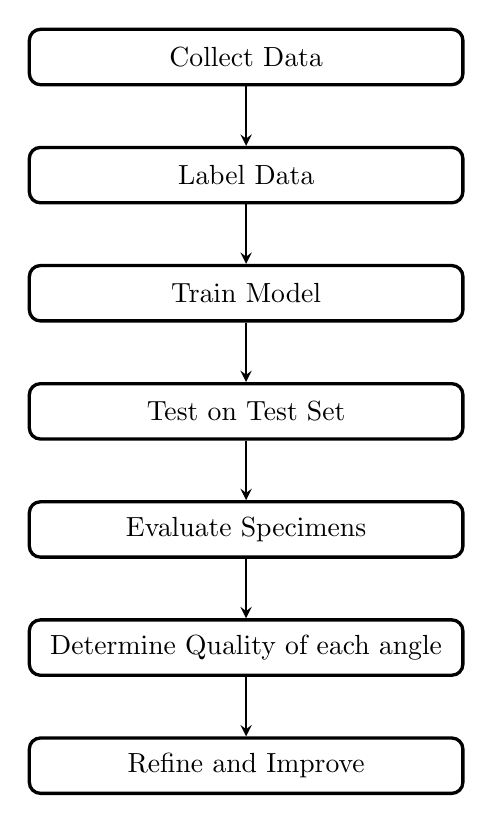
\begin{tikzpicture}[node distance=1.5cm,
    box/.style={
        rectangle,
        rounded corners,
        draw=black, very thick,
        text width=15em,
        minimum height=2em,
        text centered},
    arrow/.style={
        thick,
        ->,
        >=stealth}
    ]

    \node (collect) [box] {Collect Data};
    \node (mix) [box, below of=collect] {Label Data};
    \node (train) [box, below of=mix] {Train Model};
    \node (test) [box, below of=train] {Test on Test Set};
    \node (evaluate) [box, below of=test] {Evaluate Specimens};
    \node (rate) [box, below of=evaluate] {Determine Quality of each angle};
    \node (improve) [box, below of=rate] {Refine and Improve};
    
    \draw [arrow] (collect) -- (mix);
    \draw [arrow] (mix) -- (train);
    \draw [arrow] (train) -- (test);
    \draw [arrow] (test) -- (evaluate);
    \draw [arrow] (evaluate) -- (rate);
    \draw [arrow] (rate) -- (improve);
    
    \end{tikzpicture}
\end{center}

\textbf{Data Collection:} Utilize a microtome to slice tissue sections that have been pre-prepared and paraffin-embedded in a biological laboratory following staining procedures. Operate the microtome according to its manual to obtain images of the sections and record the cutting parameters.

\textbf{Data Labeling:} Label the collected image data based on the quality of the sections and their suitability for biological observation and analysis.

\textbf{Model Training:} Experiment with various structures and forms of deep learning convolutional models to train the labeled data. Monitor accuracy and loss functions during the training process to assess model performance.

\textbf{Testing with Test Set:} Evaluate the trained model using a test set to assess its generalization capability.

\textbf{Specimen Evaluation:} Assess an additional prepared test set to observe the practical application effects of the model, calculating the model’s prediction accuracy.

\textbf{Determination of Cutting Yield:} Use pre-prepared image data of sections cut at different angles to evaluate with the model, deriving the yield of good cuts at various angles to determine the optimal cutting angle.

\textbf{Improvements and Enhancements:} Based on the evaluation results, adjust and enhance the model to improve its accuracy and generalization capabilities.

\subsection{Image Processing Methods}

For the acquired image data, appropriate image preprocessing can be applied. Under the premise of maintaining the integrity and quality of images, certain processing can be implemented to highlight the features intended for computer recognition and, to some extent, remove irrelevant features and noise. This enhances the accuracy of subsequent deep learning models.

Image segmentation is a critical step in image processing, aiming to divide the image into several meaningful regions for further analysis and processing. In models focusing on the yield rate of biological tissues, it is necessary to segment the biological sections into biological tissue and paraffin areas, emphasizing the biological tissue parts.

Common image segmentation algorithms include edge detection and threshold segmentation.

\subsubsection{Edge Detection for Tissue Slices}
For biological tissue sections, a crucial indicator of quality is the clarity of the section's edges. The integrity and continuity of the slice edges can reflect whether there are quality issues with the sample.

There are numerous algorithms for edge detection, such as Sobel, Laplacian, and Canny operators \cite{3.1}.

The \textbf{Sobel operator} is a first-order differential operator that can be used to detect image edges \cite{补充1}. Suppose there is a one-dimensional image $f(x)$, the relationship between its intensity and the pixel coordinate $x$ can be represented as shown in Figure 1. It can be observed in \autoref{fig:original_function} that the slope is the largest around x=2.2, indicating that there is a sudden change in image intensity (an edge exists) near this point. Taking its derivative gives the first-order derivative $f'(x)$, as shown in \autoref{fig:first_derivative}, where the absolute value of the derivative is the largest. The Sobel operator uses this characteristic to detect edges.

\begin{figure}[htbp]
    \centering
    \begin{minipage}[b]{0.32\textwidth}
        \centering
        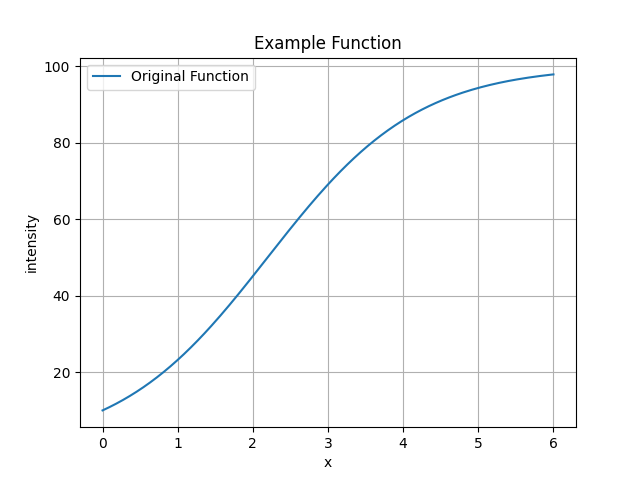
\includegraphics[width=\textwidth]{./fig/original_function.png}
        \caption{f(x)}
        \label{fig:original_function}
    \end{minipage}
    \begin{minipage}[b]{0.32\textwidth}
        \centering
        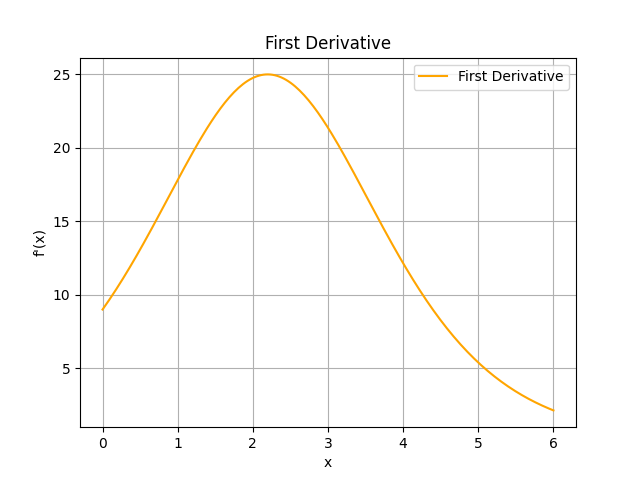
\includegraphics[width=\textwidth]{./fig/first_derivative.png}
        \caption{f'(x)}
        \label{fig:first_derivative}
    \end{minipage}
    \begin{minipage}[b]{0.32\textwidth}
        \centering
        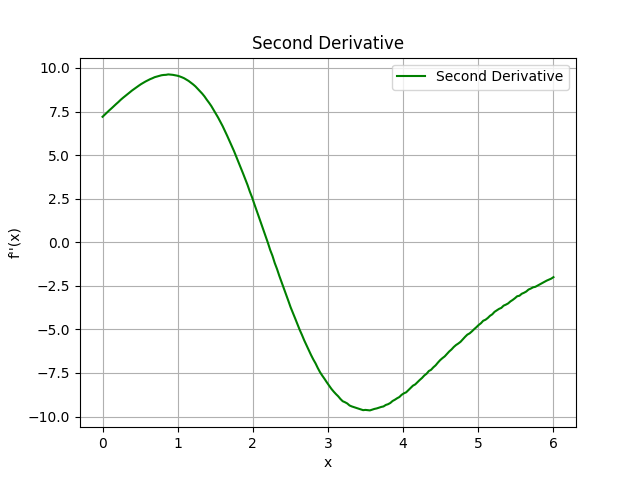
\includegraphics[width=\textwidth]{./fig/second_derivative.png}
        \caption{f''(x)}
        \label{fig:second_derivative}
    \end{minipage}
\end{figure}

The \textbf{Laplacian operator} is a second-order differential operator that performs well in edge detection of images. It is derived by taking the derivative of the Sobel operator once more. In 2D images, the Laplacian operator is defined as follows: 

\begin{equation} 
    \nabla^2 f = \frac{\partial^2 f}{\partial x^2} + \frac{\partial^2 f}{\partial y^2} 
\end{equation} 

As shown in the figure above, taking the derivative of the first-order derivative results in the second-order derivative $f''(x)$, as shown in \autoref{fig:second_derivative}. It can be seen that around x=2.2, the second-order derivative is 0, which indicates that when the value of the Laplacian operator $\nabla^2 f$ is 0, there is a sudden change in image intensity, indicating the presence of an edge.

\textbf{Canny Operator} is a multi-stage differential operator that enhances the edge detection process by incorporating noise suppression, building on the initial computations similar to those used by the Sobel operator. Introduced by John F. Canny in 1986 \cite{3.2}, the Canny operator refines the results obtained from Sobel operator calculations through additional steps such as non-maximum suppression and hysteresis thresholding. These steps set thresholds to eliminate false edges from the image, resulting in more accurate edge detection.

In the section on "Experimental Work/Analytical Investigation/Design", experiments will be conducted on the collected image data using these three edge detection algorithms—Sobel, Laplacian, and Canny—to compare their effectiveness. This comparative analysis will help in identifying the most suitable method for edge detection in the context of tissue sectioning, where the clarity and precision of edges are vital for quality assessment. The results will guide the selection of the optimal algorithm to be integrated into the image processing pipeline, enhancing the capability of the system to accurately segment and analyze biological tissue sections.

\subsubsection{Theresold Segmentation for Tissue Slices}

Apart from edge detection, another method employed is threshold segmentation. This technique divides the image pixels into two categories: those above a certain threshold and those below it. It is particularly useful in situations where there is a significant grayscale difference between the target and the background in the image.

For specimens, a straightforward approach is to contrast the colors of the paraffin area and the biological tissue area (which is stained during preparation), and then separate them using threshold segmentation. Assuming the biological tissue is yellow and the paraffin is white, setting a threshold could isolate the white parts of the image, leaving behind the biological tissue.

Additionally, there are more sophisticated methods of threshold segmentation, such as the Otsu method used for fingerprint extraction. Implementing this method can significantly enhance the segmentation of biological tissues. Yue Yaru and Zhu Jialin in "Algorithm of fingerprint extraction and implementation based on OpenCV" have proposed an improved Otsu-based fingerprint extraction algorithm using OpenCV. This algorithm excels particularly under conditions of uneven illumination and blurred images, providing accurate, simple, and fast fingerprint extraction \cite{3.3}.

Comparisons and experiments related to these segmentation techniques will be conducted in the "Experimental Work/Analytical Investigation/Design" section.

\subsection{Simple Convolutional Neural Network Framework}

Based on the design of convolutional neural network architectures discussed in the literature review, a simple convolutional neural network framework is suitable for classifying images of biological tissue sections in this project. We have constructed three simple convolutional neural network models, labeled as configurations a, b, and c.

Each of these models features a distinct combination of convolutional layers and neuron numbers in both the convolutional and fully connected layers, as summarized in the table below:

\begin{table}[H]
    \centering
    \caption{Configuration of the simple CNN model}
    \begin{tabular}{ccccc}
        \toprule
        \textbf{Layer Type} & \textbf{Configuration a} & \textbf{Configuration b} & \textbf{Configuration c} \\
        \midrule
        Input Layer & - & - & - \\
        Conv Layer 1 & Conv3-32 (relu) & Conv3-16 (relu) & Conv3-32 (relu) \\
        Pooling Layer 1 & MaxPooling & MaxPooling& MaxPooling \\
        Conv Layer 2 & Conv3-32 (relu) & Conv3-32 (relu) & Conv3-32 (relu) \\
        Pooling Layer 2 & MaxPooling & MaxPooling& MaxPooling \\
        Conv Layer 3 & Conv3-32 (relu) & Conv3-64 (relu) & Conv3-32 (relu) \\
        Pooling Layer 3 & MaxPooling & MaxPooling& MaxPooling \\
        Flattening Layer & Flatten() & Flatten() & Flatten() \\
        FC(Full connect) & Dense(128, relu) & Dense(128, relu) & Dense(256, relu) \\
        Output Layer & - & - & - \\
        \bottomrule
    \end{tabular}
    \label{tab:cnn_simple_configuration}
    \end{table}

Model a consists of three convolutional layers with 32 neurons each and a fully connected layer with 128 neurons. Model b features three convolutional layers with a progressively increasing number of neurons (16, 32, and 64), and a fully connected layer with 128 neurons. Model c also includes three convolutional layers, each with 32 neurons, but differs in its fully connected layer, which contains 256 neurons.

The primary differences among these models lie in the number of neurons in the convolutional and fully connected layers. In the "Experimental Work/Analytical Investigation/Design" section, these models will be subjected to experiments and performance evaluations to compare their effectiveness.

\subsection{Model Selection of Transfer Learning Methods}
In transfer learning, commonly used pre-trained models include VGG16, VGG19, Inception, and others. These models have been extensively trained on large datasets like ImageNet, where the weights of various layers in the model have been optimized and can be effectively used for transfer learning\cite{4.30 7}.

\autoref{tab:model_comparison} displays the number of parameters for models such as the VGG series (VGG16, VGG19) designed by the Visual Geometry Group at the University of Oxford \cite{DL.5}, as well as the modular deep learning models InceptionV3 \cite{DL.6}\cite{DL.7} developed by Google. These models possess a vast quantity of parameters, enabling them to accurately extract features from complex images. Utilizing the capabilities of these well-trained models allows researchers and practitioners to achieve high performance on specific tasks without the need to train the entire network from scratch, thereby saving time and resources while maintaining high accuracy\cite{4.30 8}.

\begin{table}[H]
    \centering
    \caption{Comparison of CNN Models}
    \label{tab:model_comparison}
    \begin{tabular}{cccc}
        \toprule
        \textbf{Model} & \textbf{VGG16} & \textbf{VGG19} & \textbf{InceptionV3}\\
        \midrule
        \textbf{Number of Parameters} & 138,357,544 & 143,667,240 & 23,851,784 \\
        \bottomrule
    \end{tabular}
\end{table}

The primary differences between these models are as follows:

\begin{itemize}
\item VGG16 (Model 3a) and VGG19 (Model 3b) are similar, but VGG19 includes three additional convolutional layers, potentially offering better feature extraction capabilities.
\item InceptionV3 (Model 3c) incorporates Inception modules, enabling it to capture a broader range of features across multiple scales, providing a more complex and possibly more effective feature extraction mechanism.
\end{itemize}

Considering that these models are all trained on the ImageNet dataset, and the features of the biological tissue slice dataset are quite different from the ImageNet dataset. As for how to determine the best model, it needs to be verified through experiments. In the section of "Experimental Work/Analytical Investigation/Design", these models will be experimented and performance evaluated, comparing their effects.






